% !TEX TS-program = knitr
\documentclass[handout]{beamer}\usepackage[]{graphicx}\usepackage[]{color}
% maxwidth is the original width if it is less than linewidth
% otherwise use linewidth (to make sure the graphics do not exceed the margin)
\makeatletter
\def\maxwidth{ %
  \ifdim\Gin@nat@width>\linewidth
    \linewidth
  \else
    \Gin@nat@width
  \fi
}
\makeatother

\definecolor{fgcolor}{rgb}{0.345, 0.345, 0.345}
\newcommand{\hlnum}[1]{\textcolor[rgb]{0.686,0.059,0.569}{#1}}%
\newcommand{\hlstr}[1]{\textcolor[rgb]{0.192,0.494,0.8}{#1}}%
\newcommand{\hlcom}[1]{\textcolor[rgb]{0.678,0.584,0.686}{\textit{#1}}}%
\newcommand{\hlopt}[1]{\textcolor[rgb]{0,0,0}{#1}}%
\newcommand{\hlstd}[1]{\textcolor[rgb]{0.345,0.345,0.345}{#1}}%
\newcommand{\hlkwa}[1]{\textcolor[rgb]{0.161,0.373,0.58}{\textbf{#1}}}%
\newcommand{\hlkwb}[1]{\textcolor[rgb]{0.69,0.353,0.396}{#1}}%
\newcommand{\hlkwc}[1]{\textcolor[rgb]{0.333,0.667,0.333}{#1}}%
\newcommand{\hlkwd}[1]{\textcolor[rgb]{0.737,0.353,0.396}{\textbf{#1}}}%
\let\hlipl\hlkwb

\usepackage{framed}
\makeatletter
\newenvironment{kframe}{%
 \def\at@end@of@kframe{}%
 \ifinner\ifhmode%
  \def\at@end@of@kframe{\end{minipage}}%
  \begin{minipage}{\columnwidth}%
 \fi\fi%
 \def\FrameCommand##1{\hskip\@totalleftmargin \hskip-\fboxsep
 \colorbox{shadecolor}{##1}\hskip-\fboxsep
     % There is no \\@totalrightmargin, so:
     \hskip-\linewidth \hskip-\@totalleftmargin \hskip\columnwidth}%
 \MakeFramed {\advance\hsize-\width
   \@totalleftmargin\z@ \linewidth\hsize
   \@setminipage}}%
 {\par\unskip\endMakeFramed%
 \at@end@of@kframe}
\makeatother

\definecolor{shadecolor}{rgb}{.97, .97, .97}
\definecolor{messagecolor}{rgb}{0, 0, 0}
\definecolor{warningcolor}{rgb}{1, 0, 1}
\definecolor{errorcolor}{rgb}{1, 0, 0}
\newenvironment{knitrout}{}{} % an empty environment to be redefined in TeX

\usepackage{alltt}
\setbeamercovered{dynamic}
\newcommand{\answers}{1}


\usetheme{Marburg}
\setbeamertemplate{navigation symbols}{} 
\setbeamertemplate{footline}
{
  \leavevmode%
  \hbox{%
  \begin{beamercolorbox}[wd=.333333\paperwidth,ht=2.25ex,dp=1ex,center]{author in head/foot}%
    \usebeamerfont{author in head/foot} $\ $ \insertshortauthor%~~\beamer@ifempty{\insertshortinstitute}{}{(\insertshortinstitute)}
  \end{beamercolorbox}%
  \begin{beamercolorbox}[wd=.333333\paperwidth,ht=2.25ex,dp=1ex,center]{title in head/foot}%
    \usebeamerfont{title in head/foot} \insertinstitute
  \end{beamercolorbox}%
  \begin{beamercolorbox}[wd=.333333\paperwidth,ht=2.25ex,dp=1ex,right]{date in head/foot}%
    \usebeamerfont{date in head/foot}\insertshortdate{}\hspace*{2em}
    \insertframenumber{} / \inserttotalframenumber\hspace*{2ex} 
  \end{beamercolorbox}}%
  \vskip0pt%
}

\usepackage{amsmath}
\usepackage{caption}
\usepackage{color}
\usepackage{enumerate}
\usepackage{listings}
\usepackage{hyperref}
\usepackage{mathrsfs}
\usepackage{natbib}
\usepackage{url}

\providecommand{\all}{\ \forall \ }
\providecommand{\bs}{\backslash}
\providecommand{\e}{\varepsilon}
\providecommand{\E}{\ \exists \ }
\providecommand{\lm}[2]{\lim_{#1 \rightarrow #2}}
\providecommand{\m}[1]{\mathbb{#1}}
\providecommand{\nv}{{}^{-1}}
\providecommand{\ov}[1]{\overline{#1}}
\providecommand{\p}{\newpage}
\providecommand{\q}{$\quad$ \newline}
\providecommand{\rt}{\rightarrow}
\providecommand{\Rt}{\Rightarrow}
\providecommand{\vc}[1]{\boldsymbol{#1}}
\providecommand{\wh}[1]{\widehat{#1}}

\hypersetup{colorlinks,linkcolor=,urlcolor=blue}
\numberwithin{equation}{section}

\definecolor{dkgreen}{rgb}{0,0.6,0}
\definecolor{gray}{rgb}{0.5,0.5,0.5}
\definecolor{mauve}{rgb}{0.58,0,0.82}

\lstset{ 
  language=C,                % the language of the code
  basicstyle= \footnotesize,           % the size of the fonts that are used for the code
  numberstyle= \tiny \color{white},  % the style that is used for the line-numbers
  stepnumber=2,                   % the step between two line-numbers. 
  numbersep=5pt,                  % how far the line-numbers are from the code
  backgroundcolor=\color{white},      % choose the background color. You must add \usepackage{color}
  showspaces=false,               % show spaces adding particular underscores
  showstringspaces=false,         % underline spaces within strings
  showtabs=false,                 % show tabs within strings adding particular underscores
  frame=lrb,                   % adds a frame around the code
  rulecolor=\color{black},        % if not set, the frame-color may be changed on line-breaks within not-black text 
  tabsize=2,                      % sets default tabsize to 2 spaces
  captionpos=t,                   % sets the caption-position 
  breaklines=true,                % sets automatic line breaking
  breakatwhitespace=false,        % sets if automatic breaks should only happen at whitespace
  %title=\lstname,                   % show the filename of files included with \lstinputlisting;
  keywordstyle=\color{blue},          % keyword style
  commentstyle=\color{gray},       % comment style
  stringstyle=\color{dkgreen},         % string literal style
  escapeinside={\%*}{*)},            % if you want to add LaTeX within your code
  morekeywords={*, ...},               % if you want to add more keywords to the set
  xleftmargin=0.053in, % left horizontal offset of caption box
  xrightmargin=-.03in % right horizontal offset of caption box
}

%\DeclareCaptionFont{white}{\color{white}}
%\DeclareCaptionFormat{listing}{\parbox{\textwidth}{\colorbox{gray}{\parbox{\textwidth}{#1#2#3}}\vskip-0.05in}}
%\captionsetup[lstlisting]{format = listing, labelfont = white, textfont = white}
%For caption-free listings, comment out the 3 lines above and uncomment the 2 lines below.
 \captionsetup{labelformat = empty, labelsep = none}
 \lstset{frame = single}



\title{Random Intervals and Confidence Intervals (Ch. 6.1)}
\author{Yifan Zhu}
\date{}
\institute{Iowa State University}
\IfFileExists{upquote.sty}{\usepackage{upquote}}{}
\begin{document}

\begin{frame}
\titlepage
 \end{frame}
 
 \AtBeginSection[]
{
   \begin{frame}
       \frametitle{Outline}
       \tableofcontents[currentsection]
   \end{frame}
}

\section{Motivation}

\begin{frame}
\frametitle{Statistical inference}
\begin{itemize}
\item {\bf Statistical inference}: using data from the sample to draw formal conclusions about the population 
\begin{itemize}
\pause \item Point estimation (confidence intervals): estimating population parameters and specifying the degree of precision of the estimate.
\pause \item Hypothesis testing: testing the validity of statements about the population that are framed in terms of parameters. 
\end{itemize}
\end{itemize}
\end{frame}


\begin{frame}
\frametitle{Motivation for confidence intervals}
\begin{itemize}
\item We want information on a population. For example:
\begin{itemize}
\pause \item True mean breaking strength of a kind of wire rope.
\pause \item True mean fill weight of food jars.
\pause \item True mean instrumental drift of a kind of scale.
\pause \item Average number of cycles to failure of a kind of spring. 
\end{itemize}
\pause \item We can use point estimates:
\begin{itemize}
\pause \item For example: if we measure breaking strengths (in tons) of 6 wire ropes as 5, 3, 7, 3,10, and 1,  we might estimate the true mean breaking strength $\mu \approx \ov{x} = \frac{5+3+7+3+10+1}{6} = 4.83$ tons.
\end{itemize}
\pause \item Or, we can use interval estimates:
\begin{itemize}
\pause \item $\mu$ is likely to be inside the interval $(4.83 - 2, 4.83 + 2) = (2.83, 6.83)$.
\pause \item We are confident that the true mean breaking strength, $\mu$, is somewhere in $(2.83, 6.83)$. But how confident can we be?
\end{itemize}
\end{itemize}
\end{frame}






\section{Random Intervals}




\begin{frame}
\frametitle{Random intervals}
\begin{itemize}
\item A {\bf random interval} is an interval on the real line with a random variable at one or both of the endpoints.
\pause \item Examples:
\begin{itemize}
\pause \item $(Z - 2, Z + 2)$, $Z \sim N(0,1)$
\pause \item $(Z, \infty)$
\pause \item $(-\infty, X)$, $X \sim N(-2, 9)$
\pause \item $(T - s \cdot t_{7, 0.975}, T + s \cdot t_{7, 0.975})$, $T \sim t_{7}$
\pause \item $(X - \sigma \cdot z_{1 - \alpha}, \infty)$, $X \sim N(5, \sigma^2), \ 0 < \alpha < 1$.
\end{itemize}
\pause \item Random intervals take into account the uncertainty in the measurement of a true mean, $\mu$. 
\end{itemize}
\end{frame}

\begin{frame}
\frametitle{Example: instrumental drift}
\begin{itemize}
\item Let $Z$ be a measure of instrumental drift of a random voltmeter that comes out of a certain factory. Say
$Z \sim N(0,1)$.
\pause \item Define a random interval:
\pause \begin{align*}
(Z - 2, Z + 2)
\end{align*}
\pause \item What is the probability that $-1$ is inside the interval?
\begin{itemize}
\pause \item Equivalent to asking how likely it is that the drift of the next instrument is within 2 units of -1.
\end{itemize}
\end{itemize}
\end{frame}

\begin{frame}
\frametitle{Example: instrumental drift}
\begin{align*}
P (-1 \text{ in } (Z - 2, Z + 2)) & \uncover<2->{= P (Z - 2 < -1 < Z + 2)} \\
&\uncover<3->{= P (Z -1 < 0 < Z + 3)} \\
&\uncover<4->{= P(-1 < -Z < 3)} \\
&\uncover<5->{= P(-3 < Z < 1)} \\
&\uncover<6->{= P(Z \le 1)-P(Z \le -3)} \\
&\uncover<7->{= \Phi(1) - \Phi(-3)} \\
&\uncover<8->{= 0.84}
\end{align*}
\end{frame}

\begin{frame}
\frametitle{Example: instrumental drift: the range of $Z$ values for which $-1$ is in $(Z - 2, Z + 2)$}
\begin{center}
\setkeys{Gin}{width=.8\textwidth} 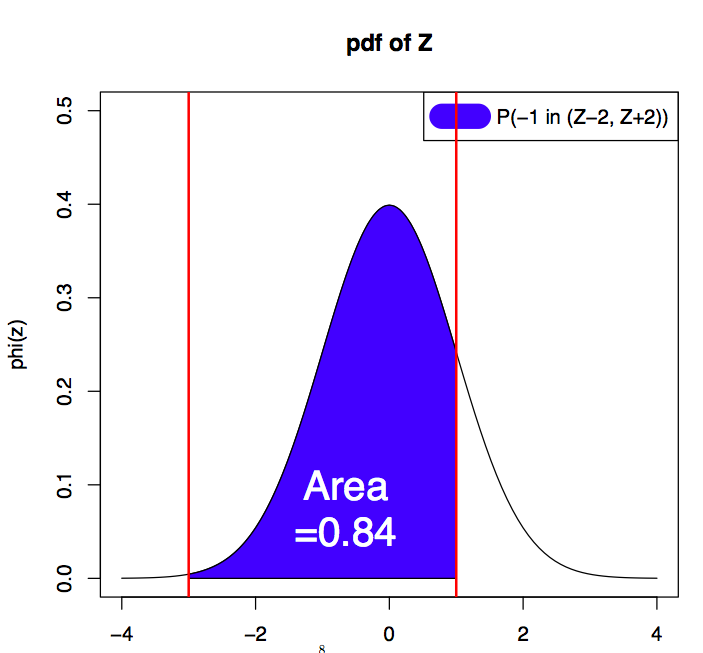
\includegraphics{../../fig/rintv1pict.png}
\end{center}
\end{frame}

\begin{frame}
\frametitle{Your turn: random intervals}
Calculate: \q
\begin{enumerate}[1. ]
\item $P(2 \text{ in } (X - 1, X + 1)), \ X \sim N(2, 4)$
\item $P(6.6 \text{ in } (X - 2, X + 1)), \ X \sim N(7, 2)$
\end{enumerate} \q
Here, $0 < \alpha < 1$.
\end{frame}

\begin{frame}<handout:\answers>
\frametitle{Answers: random intervals}
\begin{enumerate}[1. ]
\item $X \sim N(2, 4)$
\begin{align*}
P(2 \in (X - 1, X + 1)) & \uncover<2->{ = P(X - 1 < 2 < X + 1)} \\
&\uncover<3->{= P(-1 < 2 - X < 1)} \\
&\uncover<4->{= P(-1 < X - 2 < 1)} \\
&\uncover<5->{=P \left ( \frac{-1}{2} < \frac{X - 2}{2} < \frac{1}{2} \right )} \\
&\uncover<6->{= P( -0.5 < Z < 0.5)} \\
&\uncover<7->{= \Phi(0.5) - \Phi(-0.5)} \\
&\uncover<8->{= 0.69 - 0.31} \\
&\uncover<9->{= 0.38}
\end{align*}
\end{enumerate}
\end{frame}

\begin{frame}<handout:\answers>
\frametitle{Answers: random intervals}
\begin{enumerate}[1. ]
\setcounter{enumi}{1}
\item $X \sim N(7, 2)$
\begin{align*}
P(6.6 \in (X - 2, X + 1)) & \uncover<2->{= P(X - 2 < 6.6 < X + 1)} \\
&\uncover<3->{= P(-2 < 6.6 - X < 1)} \\
&\uncover<4->{ = P(-1 < X - 6.6 < 2)} \\
&\uncover<5->{ = P(-1.4 < X - 7 < 1.6)} \\
&\uncover<6->{=P \left (\frac{-1.4}{\sqrt{2}} < \frac{X - 7}{\sqrt{2}} < \frac{1.6}{\sqrt{2}} \right ) }\\
&\uncover<7->{= P( -0.99 < Z < 1.13)} \\
&\uncover<8->{= \Phi(1.13) - \Phi(-0.99)} \\
&\uncover<9->{= 0.87 - 0.16} \\
&\uncover<10->{= 0.71}
\end{align*}
\end{enumerate}
\end{frame}





\begin{frame}
\frametitle{More abstract random intervals} \scriptsize
\begin{itemize}
\item Let's say $X_1, X_2, \ldots, X_n$ are iid with:
\begin{itemize}
\pause \item $n \ge 25$
\pause \item mean $\mu$
\pause \item variance $\sigma^2$
\end{itemize}
\pause \item The random interval, $(\ov{X} - z_{1-\alpha} \frac{\sigma}{\sqrt{n}}, \  \infty)$, is useful for estimating $\mu$ ($0 < \alpha < 1)$.
\pause \item The interval contains $\mu$ with probability $1 - \alpha$.
\begin{align*}
\uncover<7->{P (\mu \in ( }&\uncover<7->{ \ov{X} - z_{1 - \alpha} \frac{\sigma}{\sqrt{n}}, \ \infty) )} \\
&\uncover<8->{= P \left (\ov{X} - z_{1 - \alpha} \frac{\sigma}{\sqrt{n}} < \mu \right)} \\
&\uncover<9->{= P \left (\ov{X} - \mu <  z_{1 - \alpha}\frac{\sigma}{\sqrt{n}} \right )} \\
&\uncover<10->{= P \left ( \frac{\ov{X} - \mu}{\sigma/\sqrt{n}} < z_{1 - \alpha} \right )} \\
&\uncover<11->{\approx P( Z < z_{1 - \alpha}) \quad \text{ \scriptsize (Central Limit Theorem)} } \\
&\uncover<12->{= \Phi(z_{1 - \alpha})} \\
&\uncover<13->{= 1 - \alpha \quad \text{\scriptsize (by the definition of $z_p$)}}
\end{align*}
\end{itemize}
\end{frame}



\begin{frame}
\frametitle{Your turn: abstract random intervals}
Calculate: \q
\begin{enumerate}[1. ]
\item $P(\mu \in (-\infty, \ \ov{X} + z_{1 - \alpha} \frac{\sigma}{\sqrt{n}})), \ \ov{X} \sim N(\mu, \sigma^2)$
\item $P(\mu \in (\ov{X} - z_{1 - \alpha/2} \frac{\sigma}{\sqrt{n}}, \ \ov{X} + z_{1 - \alpha/2} \frac{\sigma}{\sqrt{n}})), \ X \sim N(\mu, \sigma^2)$
\end{enumerate} \q

Remember the Central Limit Theorem:
\begin{align*}
\frac{\ov{X} - \mu}{\sigma/\sqrt{n}} \approx N(0,1)
\end{align*}

\end{frame}


\begin{frame}<handout:\answers>
\frametitle{Answers: abstract random intervals}
\begin{enumerate}

\item
\begin{align*}
P(\mu \in &(-\infty, \ \ov{X} + z_{1 - \alpha} \frac{\sigma}{\sqrt{n}})) \\
&\uncover<2->{= P\left ( \mu <  \ov{X} + z_{1 - \alpha} \frac{\sigma}{\sqrt{n}}\right)} \\
&\uncover<3->{= P\left (- z_{1 - \alpha} \frac{\sigma}{\sqrt{n}} < \ov{X} - \mu \right )} \\
&\uncover<4->{ = P \left (- z_{1 - \alpha} < \frac{\ov{X} - \mu}{\sigma/\sqrt{n}} \right )} \\
&\uncover<5->{\approx P\left (-z_{1 - \alpha} < Z \right) \quad \text{\scriptsize (Central Limit Theorem)}} \\
&\uncover<6->{ = 1 - P(Z \le -z_{1-\alpha})} \\
&\uncover<7->{= 1 - \Phi(-z_{1 - \alpha})} \\
&\uncover<8->{= 1 - \Phi(z_{\alpha}) \quad \text{\scriptsize(by symmetry: N(0,1) pdf)}} \\
&\uncover<9->{= 1 - \alpha \quad \text{\scriptsize (by the definition of $z_p$)}}
\end{align*}
\end{enumerate}
\end{frame}

\begin{frame}<handout:\answers>
\frametitle{Answers: abstract random intervals}
\begin{enumerate}
\setcounter{enumi}{1}
\item  \scriptsize
\begin{align*}
P(\mu \in (X &- z_{1 - \alpha/2} \frac{\sigma}{\sqrt{n}}, \ \ov{X} + z_{1 - \alpha/2} \frac{\sigma}{\sqrt{n}})) \\
&\uncover<2->{= P \left (\ov{X} - z_{1 - \alpha/2} \frac{\sigma}{\sqrt{n}} < \mu <  \ov{X} + z_{1 - \alpha/2} \frac{\sigma}{\sqrt{n}} \right)} \\
&\uncover<3->{= P \left ( - z_{1 - \alpha/2} \cdot \frac{\sigma}{\sqrt{n}} < \mu - \ov{X} <   z_{1 - \alpha/2} \frac{\sigma}{\sqrt{n}} \right)} \\
&\uncover<4->{= P\left ( - z_{1 - \alpha/2} \frac{\sigma}{\sqrt{n}} < \ov{X} - \mu <   z_{1 - \alpha/2} \frac{\sigma}{\sqrt{n}} \right)} \\
&\uncover<5->{= P \left ( - z_{1 - \alpha/2} < \frac{\ov{X}-\mu}{\sigma/\sqrt{n}} <   z_{1 - \alpha/2} \right )} \\
&\uncover<6->{\approx P( - z_{1 - \alpha/2} < Z <   z_{1 - \alpha/2}) \quad \text{(Central Limit Theorem)}}\\
&\uncover<7->{= \Phi(z_{1 - \alpha/2}) - \Phi(-z_{1-\alpha/2})} \\
&\uncover<8->{= \Phi(z_{1 - \alpha/2}) - \Phi(z_{\alpha/2}) \quad \text{\scriptsize(by symmetry: N(0,1) pdf)}} \\
&\uncover<9->{= (1 - \frac{\alpha}{2}) - \frac{\alpha}{2}} \uncover<10->{= 1 - \alpha} \\
\end{align*}
\end{enumerate}
\end{frame}






\section{Confidence Intervals ($n \ge 25, \ \sigma$ known)}

\begin{frame}
\frametitle{Confidence intervals}
\begin{itemize}
\item A $1 - \alpha$ {\bf confidence interval} for an unknown parameter is the finite realization of a random interval that contains that parameter with probability $1 - \alpha$. 
\pause \item $1 - \alpha$ is called the {\bf confidence level} of the interval.
\pause \item Example: for observations $x_1, x_2, \ldots x_n$ from random variables $X_1, X_2, \ldots, X_n$ iid with $E(X_1) = \mu$, $Var(X_1) = \sigma^2$, a $1 - \alpha$ confidence interval for $\mu$ is:
 \begin{align*}
\uncover<4->{ \left (\ov{x}  - z_{1 - \alpha/2} \frac{\sigma}{\sqrt{n}}, \ov{x} + z_{1 - \alpha/2} \frac{\sigma}{\sqrt{n}} \right )}
\intertext{\uncover<5->{which is a random draw from the random interval:}}
\uncover<6->{ \left (\ov{X}  - z_{1 - \alpha/2} \frac{\sigma}{\sqrt{n}}, \ov{X} + z_{1 - \alpha/2} \frac{\sigma}{\sqrt{n}} \right)}
\end{align*}
\end{itemize}
\end{frame}



\begin{frame}
\frametitle{Confidence intervals for $\mu$: $\sigma$ known, $n \ge 25$}
\begin{itemize}
 \item Two-sided $1- \alpha$ confidence interval:
\pause \begin{align*}
\left (\ov{x}  - z_{1 - \alpha/2} \frac{\sigma}{\sqrt{n}}, \ov{x} + z_{1 - \alpha/2} \frac{\sigma}{\sqrt{n}} \right)
\end{align*}
\pause \item One-sided $1 - \alpha$ {\bf upper confidence interval}:
\pause \begin{align*}
\left (-\infty, \ \ov{x} + z_{1 - \alpha} \frac{\sigma}{\sqrt{n}} \right )
\end{align*}
\pause \item One-sided $1 - \alpha$ {\bf lower confidence interval}:
\pause \begin{align*}
\left (\ov{x}  - z_{1 - \alpha} \frac{\sigma}{\sqrt{n}}, \ \infty \right )
\end{align*}
\end{itemize}
\end{frame}

\begin{frame}
\frametitle{Example: fill weight of jars} \small
\begin{itemize}
\item Suppose a manufacturer fills jars of food using a stable filling process with a known standard deviation of $\sigma = 1.6 g$. 
\pause \item We take a sample of $n = $47 jars and measure the sample mean weight $\ov{x} = 138.2$ g.
\pause \item A two-sided 90\% confidence interval ($\alpha = 0.1$) for the true mean weight $\mu$ is:
\begin{align*}
&\uncover<4->{ \left (\ov{x}  - z_{1 - 0.1/2} \frac{\sigma}{\sqrt{n}}, \ \ov{x} + z_{1 - 0.1/2} \frac{\sigma}{\sqrt{n}} \right )} \\
&\uncover<5->{= \left (138.2 - z_{0.95} \frac{1.6}{\sqrt{47}}, \ 138.2 + z_{0.95} \frac{1.6}{\sqrt{47}} \right)} \\
&\uncover<6->{= \left (138.2 - 1.64 \cdot 0.23, \ 138.2 + 1.64 \cdot 0.23 \right )} \\
&\uncover<7->{= (137.82, 138.58)}
\intertext{\uncover<8->{I could have also written the interval as:}}
&\uncover<9->{ 138.2 \pm 0.38 \ g} \\
\end{align*}
\end{itemize}
\end{frame}


\begin{frame}
\frametitle{Interpreting the confidence interval: fill weight of jars}
\begin{itemize}
\item We are 90\% confident that the true mean fill weight is between 137.82g and 138.58g.
\pause \item If we took 100 more samples of 47 jars each, roughly 90 of those samples would yield confidence intervals containing the true mean fill weight.
\pause \item These methods of interpretation generalize to all confidence intervals.
\end{itemize}

\end{frame}

\begin{frame}
\frametitle{Example: fill weight of jars. }

\begin{itemize}
\item What if we just want to be sure that the true mean fill weight is high enough? 
\pause \item Then, we would use a one-side lower 90\% confidence interval:
\begin{align*}
& \uncover<3->{ \left (\ov{x}  - z_{1 - \alpha} \frac{\sigma}{\sqrt{n}}, \ \infty \right)} \\
& \uncover<4->{= \left (138.2 - z_{1 - \alpha} \frac{\sigma}{\sqrt{n}}, \ \infty \right)} \\
&\uncover<5->{= \left (138.2 - z_{0.9} \frac{1.6}{\sqrt{47}}, \ \infty \right)} \\
&\uncover<6->{= (138.2 - 1.28 \cdot 0.23, \ \infty)} \\
& \uncover<7->{= (137.91, \ \infty)}
\end{align*}
\uncover<8->{\item We're 90\% confident that the true mean fill weight is above 137.91 g.}
\end{itemize}
\end{frame}

\begin{frame}
\frametitle{Your turn: car engines}
\begin{itemize}
\item Consider a grinding process used to rebuild car engines, which involves grinding rod journals for engine crankshafts. 
\pause \item Of interest is the deviation of the true mean rod journal diameter from the target diameter.
\pause \item Suppose the standard deviation of the individual differences from the target diameter is $0.7 \times 10^{-4}$ in.
\pause \item 32 consecutive rod journals are ground, with a sample mean deviation of $-0.16 \times 10^{-4}$ in from the target diameter.
\pause \item Calculate and interpret a two-sided 95\% confidence interval for the true mean deviation from the target diameter. Is there enough evidence that we're missing the target on average?
\end{itemize}
\end{frame}

\begin{frame}<handout:\answers>
\frametitle{Answer: car engines} \scriptsize
\begin{itemize}
\item $\alpha = 1 - 0.95 = 0.05$\uncover<2->{, $n = 32$}\uncover<3->{, $\sigma = 0.7 \times 10^{-4}$}\uncover<4->{, and $\ov{x} = -0.16 \times 10^{-4}$.}
\uncover<5->{\item Interval:}
\begin{align*}
&\uncover<6->{\left (\ov{x}  - z_{1 - 0.05/2} \frac{\sigma}{\sqrt{n}}, \ \ov{x} + z_{1 - 0.05/2} \frac{\sigma}{\sqrt{n}}\right)} \\
&\uncover<7->{= \left ( -0.16 \times 10^{-4} - z_{0.975} \frac{0.7 \times 10^{-4}}{\sqrt{32}}, \  -0.16 \times 10^{-4} + z_{0.975} \frac{0.7 \times 10^{-4}}{\sqrt{32}} \right)} \\
&\uncover<8->{= ( -0.16 \times 10^{-4} -1.96 \cdot 1.2 \times 10^{-5}, \  -0.16 \times 10^{-4} + 1.96 \cdot 1.2 \times 10^{-5})} \\
&\uncover<9->{= (-4.0 \times 10^{-5}, 7.5 \times 10^{-6})}
\end{align*}
\uncover<10->{\item We are 95\% confident that the true mean deviation from the target diameter of the rod journals is between $-4.0 \times 10^{-5}$ in and $7.5 \times 10^{-6}$ in.}
\uncover<11->{\item Since 0 is in the confidence interval, there is not enough evidence to conclude that the rod journal grinding process is off target.}
\end{itemize}
\end{frame}

\begin{frame}
\frametitle{Your turn: hard disk failures} \scriptsize
\begin{itemize}
\item F. Willett, in the article \emph{The Case of the Derailed Disk Drives} (Mechanical Engineering, 1988), discusses a study done to isolate the cause of \emph{blink code A failure} in a model of Winchester hard disk drive. 
\pause \item For each disk, the investigator measured the breakaway torque (in. oz.) required to loosen the drive's interrupter flag on the stepper motor shaft.
\pause \item Breakaway torques for 26 disk drives were recorded, with a sample mean of 11.5 in. oz.
\pause \item Suppose you know the true standard deviation of the breakaway torques is $5.1$ in. oz.
\pause \item Calculate and interpret:
\begin{enumerate}[1. ]
\pause \item A two-sided 90\% confidence interval for the true mean breakaway torque of the relevant type of Winchester drive.
\pause \item An analogous two-sided 95\% confidence interval. 
\pause \item An analogous two-sided 99\% confidence interval. 
\end{enumerate}
\pause \item Is there enough evidence to conclude that the mean breakaway torque is different from the factory's standard of 33.5 in. oz.?
\end{itemize}
\end{frame}



\begin{frame}<handout:\answers>
\frametitle{Answers: hard disk failures}
\begin{itemize}
\item $\sigma = 5.1, \ov{x} = 11.5, n = 26$.
\pause \item All three confidence intervals have the form:

\begin{align*}
&\uncover<3->{\left (\ov{x}  - z_{1 - \alpha/2} \frac{\sigma}{\sqrt{n}}, \ \ov{x} + z_{1 - \alpha/2} \frac{\sigma}{\sqrt{n}} \right )} \\
&\uncover<4->{= \left (11.5 - z_{1 - \alpha/2} \frac{5.1}{\sqrt{26}}, \ 11.5 + z_{1 - \alpha/2} \frac{5.1}{\sqrt{26}} \right )} \\
&\uncover<5->{= (11.5 - 1.0002 \cdot z_{1 - \alpha/2}, \ 11.5 + 1.0002 \cdot z_{1 - \alpha/2})}
\end{align*}

\uncover<6->{\item The confidence intervals are thus:}
\begin{enumerate}[1. ]
\uncover<7->{\item $90\%$ CI means $\alpha = 0.1$}
\begin{align*}
&\uncover<8->{(11.5 - 1.0002 \cdot z_{1 - 0.1/2}, \ 11.5 + 1.0002\cdot z_{1 - 0.1/2})} \\
&\uncover<9->{= (11.5 - 1.0002\cdot z_{0.95}, \ 11.5 + 1.0002 \cdot z_{0.95})} \\
&\uncover<10->{= (11.5 - 1.0002 \cdot 1.64, \ 11.5 + 1.0002 \cdot 1.64)} \\
&\uncover<11->{= (9.86, 13.14)}
\end{align*}
\end{enumerate}
\end{itemize}
\end{frame}



\begin{frame}<handout:\answers>
\frametitle{Answers: hard disk failures}
\begin{enumerate}[1. ]
\setcounter{enumi}{1}
\item $95\%$ CI means $\alpha = 0.05$
\begin{align*}
&\uncover<2->{(11.5 - 1.0002 \cdot z_{1 - 0.05/2}, \ 11.5 + 1.0002\cdot z_{1 - 0.05/2})} \\
&\uncover<3->{= (11.5 - 1.0002\cdot z_{0.975}, \ 11.5 + 1.0002 \cdot z_{0.975})} \\
&\uncover<4->{= (11.5 - 1.0002 \cdot 1.96, \ 11.5 + 1.0002 \cdot 1.96)} \\
&\uncover<5->{= (9.54, 13.46)}
\end{align*}

\uncover<6->{\item $99\%$ CI means $\alpha = 0.01$}
\begin{align*}
&\uncover<7->{(11.5 - 1.0002 \cdot z_{1 - 0.01/2}, \ 11.5 + 1.0002\cdot z_{1 - 0.01/2})} \\
&\uncover<8->{= (11.5 - 1.0002\cdot z_{0.995}, \ 11.5 + 1.0002 \cdot z_{0.995})} \\
&\uncover<9->{= (11.5 - 1.0002 \cdot 2.33, \ 11.5 + 1.0002 \cdot 2.33)} \\
&\uncover<10->{= (9.17, 13.83)}
\end{align*}
\end{enumerate}
\end{frame}

\begin{frame}<handout:\answers>
\frametitle{Answers: hard disk failures}
\begin{itemize}
\item Notice: the confidence intervals get wider as the confidence level $1- \alpha$ increases.
\pause \item None of these confidence intervals contains the manufacturer's target of $33.5$ in. oz., so there is significant evidence that the process misses this target. 
\pause \item Hence, there is a design flaw in the manufacturing process of the disk drives that must be corrected.
\end{itemize}
\end{frame}








\begin{frame}
\frametitle{Controlling the width of a confidence interval} \small
\begin{itemize}
\item If you want to estimate the breakaway torque with a 2-sided, 95\% confidence interval with $\pm 2.0$ in. oz. of precision, what sample size would you need?
\pause \item The confidence interval is:
\begin{align*}
&\uncover<3->{\left (\ov{x}  - z_{1 - \alpha/2} \frac{\sigma}{\sqrt{n}}, \ \ov{x} + z_{1 - \alpha/2} \frac{\sigma}{\sqrt{n}} \right )} \\
&\uncover<4->{= \left (11.5 - z_{1 - 0.05/2} \cdot \frac{5.1}{\sqrt{n}} , \ 11.5 + z_{1 - 0.05/2} \cdot \frac{5.1}{\sqrt{n}} \right )} \\
&\uncover<5->{= \left (11.5 - z_{0.975} \cdot \frac{5.1}{\sqrt{n}} , \ 11.5 + z_{0.975} \cdot \frac{5.1}{\sqrt{n}} \right )} \\
&\uncover<6->{=(11.5 - 1.96 \cdot 5.1 \cdot n^{-1/2}, 11.5 + 1.96 \cdot 5.1 \cdot n^{-1/2})} \\
&\uncover<7->{=(11.5 - 9.996 \cdot n^{-1/2}, 11.5 + 9.996 \cdot n^{-1/2})} \\
\end{align*}
\end{itemize}
\end{frame}

\begin{frame}
\frametitle{Controlling the width of a confidence interval}
\begin{align*}
\intertext{\uncover<2->{The interval precision (half-width) $\delta$ is:}}
\uncover<3->{\delta} & \uncover<3->{= \frac{1}{2} \left ( (11.5 + 9.996 \cdot n^{-1/2}) - (11.5 - 9.996 \cdot n^{-1/2}) \right )} \\
&\uncover<4->{= 9.996 \cdot n^{-1/2}}
\intertext{\uncover<5->{We require $\delta$ to be at most 2:}}
\uncover<5->{2.0} & \uncover<5->{\le 9.996 \cdot n^{-1/2}} \\
\uncover<6->{n} & \uncover<6->{\ge 25}
\end{align*}
\begin{itemize}
\uncover<7->{\item We would need a sample of 25 disk drives to meet a precision of $\pm 2.0$.}
\end{itemize}
\end{frame}


\end{document}
